\titleformat {\chapter} {\normalfont\huge\bfseries\color{black}}   {\thechapter}{10pt}{\huge} 
\chapter {Simulation Results}

%% ================================
%% \input{Advice-on-Chapter-4}
%% ================================
	
\section{The Parametric Equations}
%% \label{sec:4.1-CNC-Research-Machine}

The images of the UMP 3-axis CNC research machine for our previous work are provided in next three figures. It is an experimental CNC router-type, that instead of a tool cutter, uses a pen to create drawings on paper in the X-Y plane. The Z-axis motion is used to raise and lower the pen. As a consequence, circular arc (G02, G03 G-Code) moves are applicable to the X and Y axes only, while linear (G01 G-Code) moves are applicable to all three X, Y and Z axes.  
\vspace*{1\baselineskip}
		

%%
%% \begin{figure}[htbp]
%% \begin{center}
%%	\frame{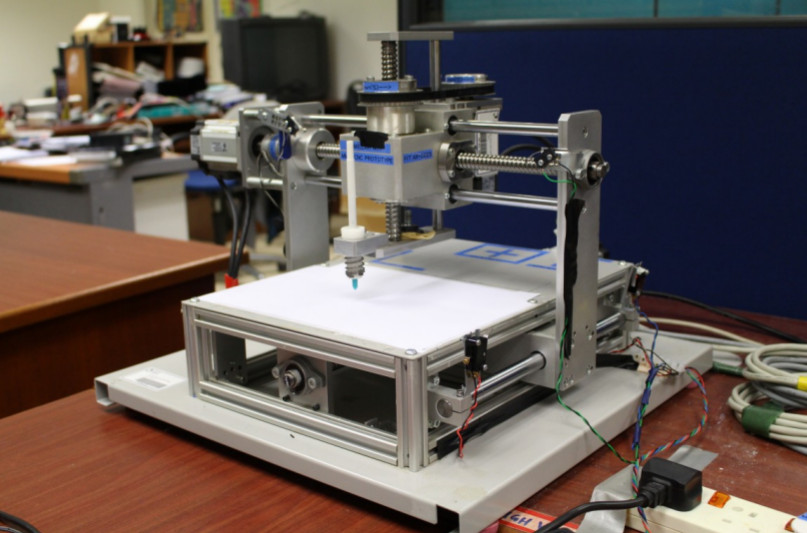
\includegraphics[width=0.85\textwidth]{./07-images/img-Ch4/CNC-Research-Machine-3-Axis.jpg}}
%%	\caption{The UMP 3-axis CNC Research Machine}
%%	\label{fig:CNC-Research-Machine-3-Axis.jpg}
%% \end{center}
%% \end{figure}

Electrical signal pulses sent to the servo-driver provide information like rotate clockwise (CW), rotate counter-clockwise(CCW), travel distance to rotate, speed to rotate, and so on. The actuation using electrical pulses makes the physical CNC machine instantaneously active. 




% ================== END CHAPTER-5 ========================